\section{Superficies}

Una superficie es un objeto bidimensional situado en el espacio. Aunque puede ser curva, alrededor de cada punto regular se parece a una porción de plano. Ejemplos habituales son los planos, las esferas, los cilindros, los conos y las gráficas de funciones de dos variables.

\begin{mydefinition}{Superficie dada como gráfica}
Sea $R\subseteq\mathbb R^2$ una región y sea $f:R\to\mathbb R$ una función continua. La gráfica de $f$ es la superficie
\[
S=\{(x,y,z)\in\mathbb R^3:(x,y)\in R,\ z=f(x,y)\}.
\]
Si $f$ tiene derivadas parciales continuas, la superficie es suave en los puntos donde el vector $\langle-f_x,-f_y,1\rangle$ está definido.
\end{mydefinition}

La región $R$ es la proyección de $S$ sobre el plano $xy$. La altura $f(x,y)$ asigna a cada punto de $R$ un único punto de la superficie. No todas las superficies son gráficas globales de la forma $z=f(x,y)$, una esfera completa, por ejemplo, requiere al menos dos gráficas o una parametrización.

\subsection{Aproximación del diferencial de superficie}

Sea $S$ la gráfica $z=f(x,y)$ sobre una región $R$ del plano $xy$. Para medir el área de $S$, primero se divide $R$ en regiones pequeñas $R_i$. Si una de ellas es aproximadamente rectangular, sus lados tienen longitudes $\Delta x_i$ y $\Delta y_i$, y su área es
\[
\Delta A_i\approx\Delta x_i\Delta y_i.
\]
Se elige un punto $(x_i^*,y_i^*)$ en $R_i$. A este punto le corresponde
\[
P_i=\bigl(x_i^*,y_i^*,f(x_i^*,y_i^*)\bigr)
\]
sobre la superficie. La porción de $S$ situada encima de $R_i$ se denota por $S_i$ y su área por $\Delta S_i$. Como $S_i$ es curva, su área no coincide en general con $\Delta A_i$.

Cuando $R_i$ es suficientemente pequeña, $S_i$ se parece a una porción del plano tangente en $P_i$. La aproximación lineal de $f$ alrededor de $(x_i^*,y_i^*)$ es
\[
z-f(x_i^*,y_i^*)
\approx f_x(x_i^*,y_i^*)(x-x_i^*)
+f_y(x_i^*,y_i^*)(y-y_i^*).
\]
Un desplazamiento de longitud $\Delta x_i$ en la dirección de $x$ produce en el plano tangente el vector
\[
\vec a_i=
\left\langle\Delta x_i,0,
f_x(x_i^*,y_i^*)\Delta x_i\right\rangle,
\]
mientras que un desplazamiento de longitud $\Delta y_i$ en la dirección de $y$ produce
\[
\vec b_i=
\left\langle0,\Delta y_i,
f_y(x_i^*,y_i^*)\Delta y_i\right\rangle.
\]
Estos vectores generan un paralelogramo tangente de área $\Delta T_i$. Como el área de un paralelogramo es la norma del producto cruz de sus lados,
\begin{align*}
\Delta T_i
&=\lVert\vec a_i\times\vec b_i\rVert\\
&=\left\lVert
\left\langle-f_x(x_i^*,y_i^*),
-f_y(x_i^*,y_i^*),1\right\rangle
\Delta x_i\Delta y_i
\right\rVert\\
&\approx
\sqrt{1+f_x(x_i^*,y_i^*)^2+f_y(x_i^*,y_i^*)^2}\,\Delta A_i.
\end{align*}
La raíz es el factor por el cual la inclinación amplía el área proyectada. Si el plano tangente es horizontal, $f_x=f_y=0$ y el factor vale $1$. Si la superficie está inclinada, el factor es mayor que $1$.

En notación diferencial, la región proyectada se representa por $dA=dx\,dy$ y el elemento correspondiente sobre la superficie por $dS$. La relación anterior se escribe
\[
dS=\sqrt{1+f_x^2+f_y^2}\,dA.
\]

\begingroup
\shorthandoff{>}
\begin{center}
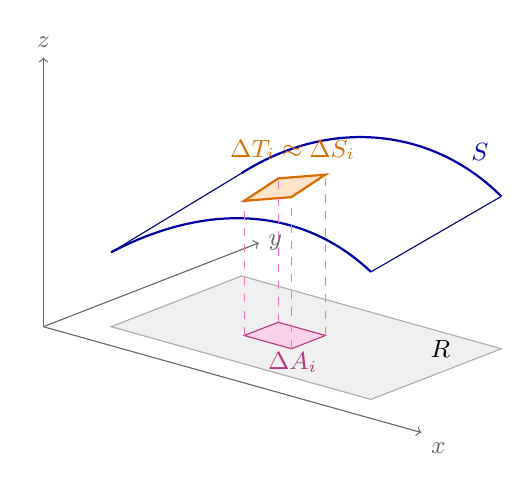
\begin{tikzpicture}[
    x={(1cm,-.28cm)},y={(.72cm,.28cm)},z={(0cm,.9cm)},
    every node/.style={font=\small}]
    \draw[->,gray!80!black] (0,0,0)--(4.8,0,0) node[below right] {$x$};
    \draw[->,gray!80!black] (0,0,0)--(0,3.8,0) node[right] {$y$};
    \draw[->,gray!80!black] (0,0,0)--(0,0,3.8) node[above] {$z$};
    \fill[gray!12] (.5,.5,0)--(3.8,.5,0)--(3.8,2.8,0)--(.5,2.8,0)--cycle;
    \draw[gray!65] (.5,.5,0)--(3.8,.5,0)--(3.8,2.8,0)--(.5,2.8,0)--cycle;
    \node at (3.35,2.35,0) {$R$};
    \draw[blue!65!black,thick] (.5,.5,1.05)
        .. controls (1.8,.4,2.2) and (3,.4,2.5) .. (3.8,.5,1.8);
    \draw[blue!65!black,thick] (.5,2.8,1.45)
        .. controls (1.7,2.7,2.65) and (3,2.7,2.9) .. (3.8,2.8,2.15);
    \draw[blue!45!black] (.5,.5,1.05)--(.5,2.8,1.45);
    \draw[blue!45!black] (3.8,.5,1.8)--(3.8,2.8,2.15);
    \fill[orange!25,opacity=.85]
        (1.65,1.25,1.9)--(2.25,1.25,2.14)--(2.25,1.85,2.27)--(1.65,1.85,2.03)--cycle;
    \draw[orange!85!black,thick]
        (1.65,1.25,1.9)--(2.25,1.25,2.14)--(2.25,1.85,2.27)--(1.65,1.85,2.03)--cycle;
    \fill[magenta!18]
        (1.65,1.25,0)--(2.25,1.25,0)--(2.25,1.85,0)--(1.65,1.85,0)--cycle;
    \draw[magenta!70!black]
        (1.65,1.25,0)--(2.25,1.25,0)--(2.25,1.85,0)--(1.65,1.85,0)--cycle;
    \draw[magenta!55,dashed] (1.65,1.25,0)--(1.65,1.25,1.9);
    \draw[magenta!55,dashed] (2.25,1.25,0)--(2.25,1.25,2.14);
    \draw[magenta!55,dashed] (2.25,1.85,0)--(2.25,1.85,2.27);
    \draw[magenta!55,dashed] (1.65,1.85,0)--(1.65,1.85,2.03);
    \node[magenta!70!black] at (2.05,1.55,-.35) {$\Delta A_i$};
    \node[orange!85!black] at (2.05,1.55,2.65) {$\Delta T_i\approx\Delta S_i$};
    \node[blue!65!black] at (3.6,2.7,2.75) {$S$};
\end{tikzpicture}
\end{center}
\endgroup

La figura compara tres cantidades: $\Delta A_i$ es el área de una región pequeña en el plano $xy$, $\Delta S_i$ es el área de la porción curva situada encima de ella, y $\Delta T_i$ es el área del paralelogramo contenido en el plano tangente. Para regiones pequeñas se tiene $\Delta S_i\approx\Delta T_i$.

La suma de las áreas de todos los paralelogramos tangentes aproxima el área total:
\begin{align*}
\operatorname{area}(S)
&\approx\sum_{i=1}^n\Delta T_i\\
&\approx\sum_{i=1}^n
\sqrt{1+f_x(x_i^*,y_i^*)^2+f_y(x_i^*,y_i^*)^2}\,\Delta A_i
\end{align*}
Al refinar la partición, el diámetro máximo de las regiones $R_i$ tiende a cero. Los planos tangentes aproximan cada vez mejor a los parches de la superficie y la suma anterior se convierte en una integral doble:
\begin{align*}
\operatorname{area}(S)
&=\lim_{\Delta A_i\to0}
\sum_{i=1}^n
\sqrt{1+f_x(x_i^*,y_i^*)^2+f_y(x_i^*,y_i^*)^2}\,\Delta A_i\\
&=\iint_R\sqrt{1+f_x^2+f_y^2}\,dA
\end{align*}
Así, la integral suma todas las contribuciones de las aproximaciones lineales para cada región pequeña de la superficie.

\newpage
\begin{mydefinition}{Área de una superficie dada como gráfica}
Sea $f$ una función con derivadas parciales continuas en una región cerrada y acotada $R$. El área de la superficie $S:z=f(x,y)$ situada sobre $R$ se define por
\[
\operatorname{area}(S)
=\iint_R\sqrt{1+f_x(x,y)^2+f_y(x,y)^2}\,dA,
\]
si la integral existe.
\end{mydefinition}

Si una superficie se expresa como $x=g(y,z)$ o $y=h(x,z)$, se proyecta sobre los planos $yz$ o $xz$, respectivamente:
\[
dS=\sqrt{1+g_y^2+g_z^2}\,dy\,dz,
\qquad
dS=\sqrt{1+h_x^2+h_z^2}\,dx\,dz.
\]

\paragraph{Ejemplo 1. Porción de un plano}
Sea $S$ la parte del plano $z=2x-y$ situada sobre el rectángulo $R=[0,1]\times[0,2]$. Para $f(x,y)=2x-y$ se tiene
\[
f_x(x,y)=2,
\qquad
f_y(x,y)=-1.
\]
Por tanto, el factor de ampliación del área es constante:
\[
\sqrt{1+f_x^2+f_y^2}=\sqrt{1+2^2+(-1)^2}=\sqrt6.
\]
La integral se evalúa primero respecto de $y$:
\begin{align*}
\operatorname{area}(S)
&=\int_0^1\int_0^2\sqrt6\,dy\,dx\\
&=\int_0^1 2\sqrt6\,dx
=2\sqrt6.
\end{align*}
El rectángulo proyectado tiene área $2$ y la inclinación del plano multiplica esa área por $\sqrt6$.

\begingroup\shorthandoff{>}
\begin{center}
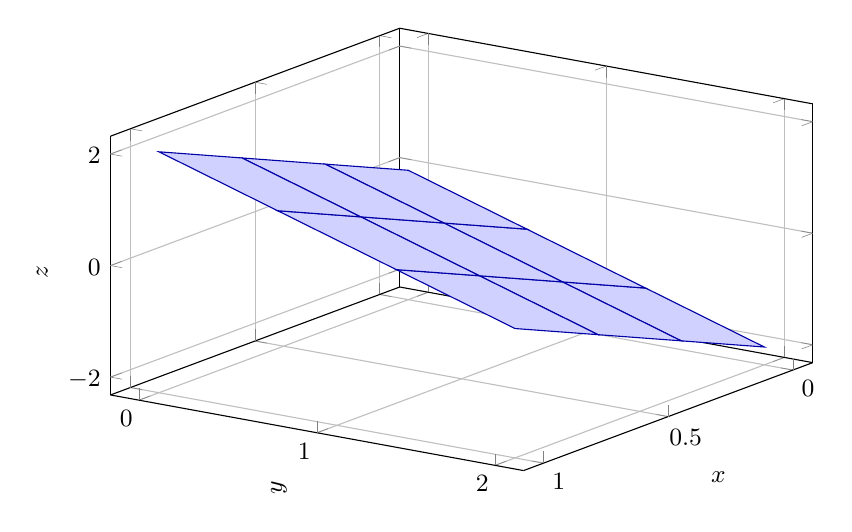
\begin{tikzpicture}
\begin{axis}[width=10.5cm,height=7.2cm,view={125}{27},axis lines=box,
    xlabel={$x$},ylabel={$y$},zlabel={$z$},domain=0:1,y domain=0:2,
    xtick={0,.5,1},ytick={0,1,2},ztick={-2,0,2},
    tick label style={font=\small},label style={font=\small},
    grid=major,enlargelimits=.08,samples=4,samples y=4,z buffer=sort]
\addplot3[surf,shader=flat,draw=blue!65!black,fill=blue!18]
    {2*x-y};
\end{axis}
\end{tikzpicture}
\end{center}
\endgroup

\paragraph{Ejemplo 2. Paraboloide sobre un disco}
Considérese $z=x^2+y^2$ sobre el disco
\[
R=\{(x,y):x^2+y^2\leq1\}.
\]
Las derivadas parciales son $f_x=2x$ y $f_y=2y$, de modo que
\[
\sqrt{1+f_x^2+f_y^2}
=\sqrt{1+4x^2+4y^2}.
\]
Como el dominio y el integrando dependen de $x^2+y^2$, se usan coordenadas polares. Con $x^2+y^2=r^2$, $dA=r\,dr\,d\theta$, $0\leq r\leq1$ y $0\leq\theta\leq2\pi$,
\begin{align*}
\operatorname{area}(S)
&=\int_0^{2\pi}\int_0^1\sqrt{1+4r^2}\,r\,dr\,d\theta\\
&=2\pi\left[\frac{(1+4r^2)^{3/2}}{12}\right]_{0}^{1}\\
&=\frac{\pi}{6}\left(5\sqrt5-1\right).
\end{align*}
En el segundo paso se utiliza la sustitución $u=1+4r^2$, para la cual $du=8r\,dr$.

\begingroup\shorthandoff{>}
\begin{center}
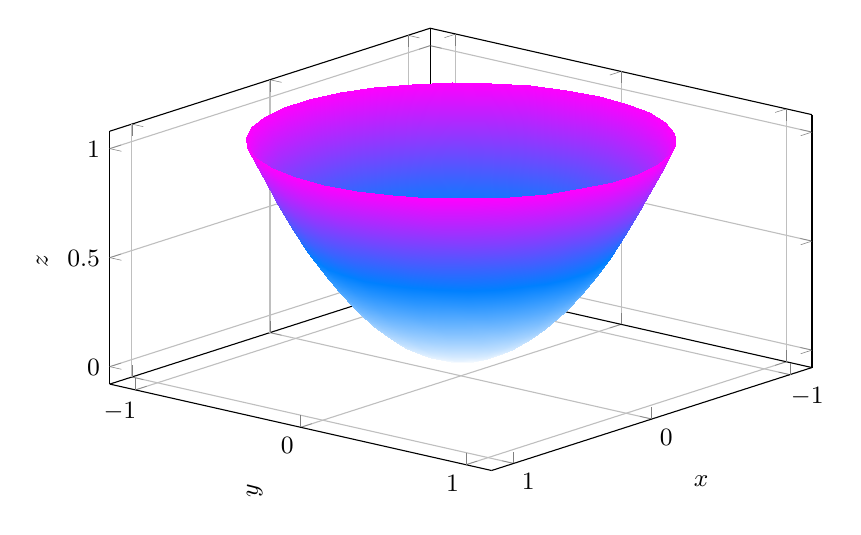
\begin{tikzpicture}
\begin{axis}[width=10.5cm,height=7.2cm,view={130}{28},axis lines=box,
    xlabel={$x$},ylabel={$y$},zlabel={$z$},domain=0:360,y domain=0:1,
    xtick={-1,0,1},ytick={-1,0,1},ztick={0,.5,1},
    tick label style={font=\small},label style={font=\small},
    grid=major,enlargelimits=.08,samples=35,samples y=15,z buffer=sort]
\addplot3[surf,shader=interp,colormap/cool]
    ({y*cos(x)},{y*sin(x)},{y^2});
\end{axis}
\end{tikzpicture}
\end{center}
\endgroup

\paragraph{Ejemplo 3. Hemisferio superior}
El hemisferio superior de radio $a$ puede escribirse como
\[
z=f(x,y)=\sqrt{a^2-x^2-y^2},
\qquad x^2+y^2\leq a^2.
\]
En los puntos interiores de su proyección,
\[
f_x=-\frac{x}{\sqrt{a^2-x^2-y^2}},
\qquad
f_y=-\frac{y}{\sqrt{a^2-x^2-y^2}}.
\]
Por consiguiente,
\[
\sqrt{1+f_x^2+f_y^2}
=\frac{a}{\sqrt{a^2-x^2-y^2}}.
\]
En coordenadas polares, $x^2+y^2=r^2$ y $dA=r\,dr\,d\theta$. Aunque el integrando crece cuando $r$ se acerca a $a$, la integral impropia converge:
\begin{align*}
\operatorname{area}(S)
&=\int_0^{2\pi}\int_0^a
\frac{ar}{\sqrt{a^2-r^2}}\,dr\,d\theta\\
&=2\pi\left[-a\sqrt{a^2-r^2}\right]_{0}^{a}\\
&=2\pi a^2.
\end{align*}
El resultado coincide con la mitad del área $4\pi a^2$ de una esfera. La figura muestra el caso $a=1$.

\begingroup\shorthandoff{>}
\begin{center}
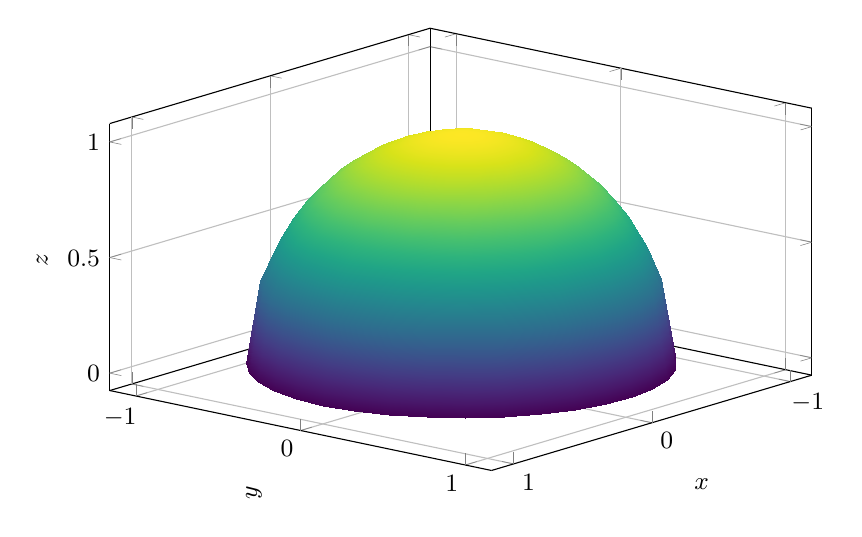
\begin{tikzpicture}
\begin{axis}[width=10.5cm,height=7.2cm,view={130}{25},axis lines=box,
    xlabel={$x$},ylabel={$y$},zlabel={$z$},domain=0:360,y domain=0:1,
    xtick={-1,0,1},ytick={-1,0,1},ztick={0,.5,1},
    tick label style={font=\small},label style={font=\small},
    grid=major,enlargelimits=.08,samples=36,samples y=16,z buffer=sort]
\addplot3[surf,shader=interp,colormap/viridis]
    ({y*cos(x)},{y*sin(x)},{sqrt(1-y^2)});
\end{axis}
\end{tikzpicture}
\end{center}
\endgroup

\paragraph{Ejemplo 4. Cilindro parabólico}
Sea $S:z=x^2$ sobre el rectángulo $0\leq x\leq1$, $0\leq y\leq2$. Puesto que $f_x=2x$ y $f_y=0$, el elemento de área es
\[
dS=\sqrt{1+4x^2}\,dA.
\]
El integrando no depende de $y$, por lo que la integración en esa variable produce el factor $2$:
\begin{align*}
\operatorname{area}(S)
&=\int_0^1\int_0^2\sqrt{1+4x^2}\,dy\,dx\\
&=2\int_0^1\sqrt{1+4x^2}\,dx.
\end{align*}
Una antiderivada necesaria es
\[
\int\sqrt{1+4x^2}\,dx
=\frac{x}{2}\sqrt{1+4x^2}
+\frac14\ln\left(2x+\sqrt{1+4x^2}\right).
\]
Por tanto,
\begin{align*}
\operatorname{area}(S)
&=2\left[
\frac{x}{2}\sqrt{1+4x^2}
+\frac14\ln\left(2x+\sqrt{1+4x^2}\right)
\right]_{0}^{1}\\
&=\sqrt5+\frac12\ln(2+\sqrt5).
\end{align*}
La superficie se extiende en la dirección de $y$ sin cambiar su perfil parabólico en el plano $xz$.

\begingroup\shorthandoff{>}
\begin{center}
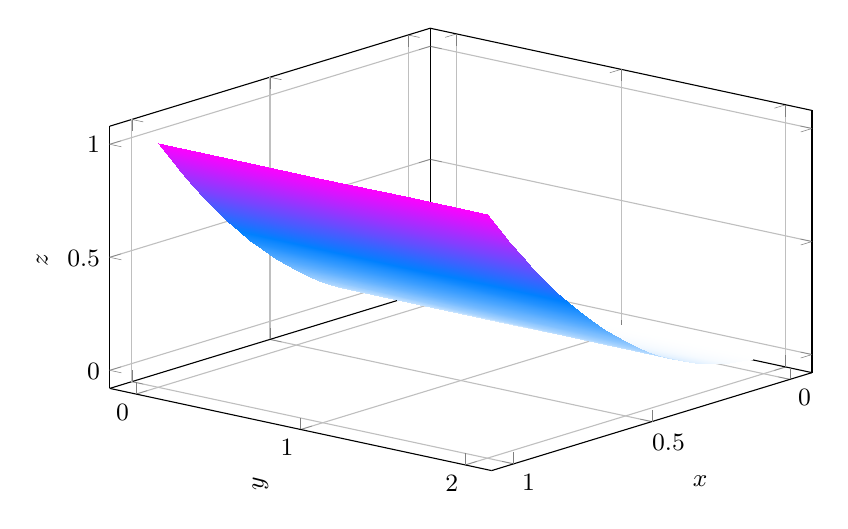
\begin{tikzpicture}
\begin{axis}[width=10.5cm,height=7.2cm,view={130}{26},axis lines=box,
    xlabel={$x$},ylabel={$y$},zlabel={$z$},domain=0:1,y domain=0:2,
    xtick={0,.5,1},ytick={0,1,2},ztick={0,.5,1},
    tick label style={font=\small},label style={font=\small},
    grid=major,enlargelimits=.08,samples=25,samples y=5,z buffer=sort]
\addplot3[surf,shader=interp,colormap/cool] {x^2};
\end{axis}
\end{tikzpicture}
\end{center}
\endgroup

\paragraph{Ejemplo 5. Cono circular}
La superficie $z=\sqrt{x^2+y^2}$ situada sobre el disco $x^2+y^2\leq a^2$ es un cono de radio $a$ y altura $a$. Para $(x,y)\neq(0,0)$,
\[
f_x=\frac{x}{\sqrt{x^2+y^2}},
\qquad
f_y=\frac{y}{\sqrt{x^2+y^2}},
\]
y, por ello,
\[
f_x^2+f_y^2
=\frac{x^2+y^2}{x^2+y^2}=1.
\]
El factor de área es entonces $\sqrt{1+f_x^2+f_y^2}=\sqrt2$. En coordenadas polares,
\begin{align*}
\operatorname{area}(S)
&=\int_0^{2\pi}\int_0^a\sqrt2\,r\,dr\,d\theta\\
&=\sqrt2\,\pi a^2.
\end{align*}
Las derivadas parciales no existen en el vértice. Para justificar el cálculo se puede excluir un disco de radio $\varepsilon$, integrar sobre $\varepsilon\leq r\leq a$ y tomar el límite cuando $\varepsilon\to0$; la contribución omitida tiende a cero. La figura muestra el caso $a=1$.

\begingroup\shorthandoff{>}
\begin{center}
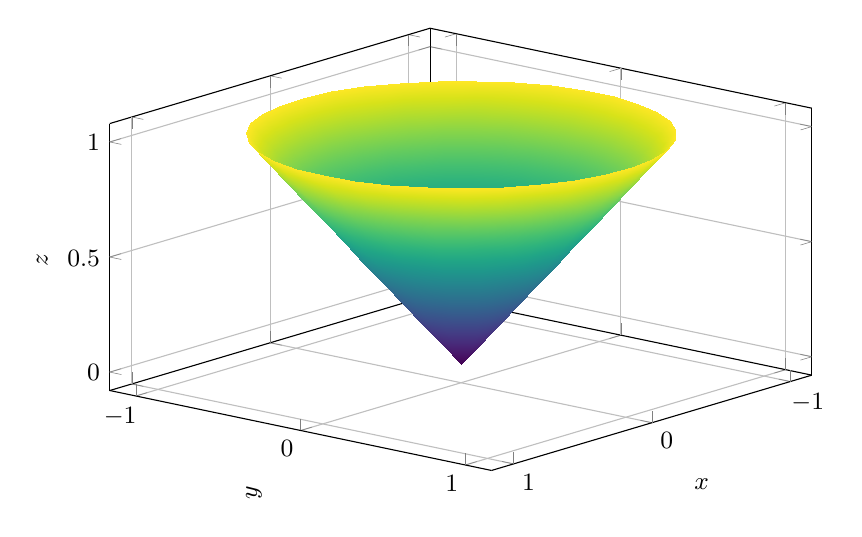
\begin{tikzpicture}
\begin{axis}[width=10.5cm,height=7.2cm,view={130}{25},axis lines=box,
    xlabel={$x$},ylabel={$y$},zlabel={$z$},domain=0:360,y domain=0:1,
    xtick={-1,0,1},ytick={-1,0,1},ztick={0,.5,1},
    tick label style={font=\small},label style={font=\small},
    grid=major,enlargelimits=.08,samples=36,samples y=12,z buffer=sort]
\addplot3[surf,shader=interp,colormap/viridis]
    ({y*cos(x)},{y*sin(x)},y);
\end{axis}
\end{tikzpicture}
\end{center}
\endgroup

\subsection{Superficies paramétricas}

Una sola ecuación cartesiana describe una superficie mediante una relación entre $x$, $y$ y $z$. Otra forma de describir superficies es mediante una parametrización, similar a como se define una curva mediante un parámetro (una dimensión), para el caso de superficies se utilizan dos parámetros (dos dimensiones).

\begin{mydefinition}{Superficie paramétrica}
Sea $D\subseteq\mathbb R^2$ un dominio con parámetros $(u,v)$. Una superficie paramétrica es la imagen de una función vectorial
\[
\vec r:D\to\mathbb R^3,
\qquad
\vec r(u,v)=\langle x(u,v),y(u,v),z(u,v)\rangle.
\]
La superficie es $S=\{\vec r(u,v):(u,v)\in D\}$. Las curvas obtenidas al mantener fijo uno de los parámetros se llaman curvas coordenadas.
\end{mydefinition}

\begingroup
\shorthandoff{>}
\begin{center}
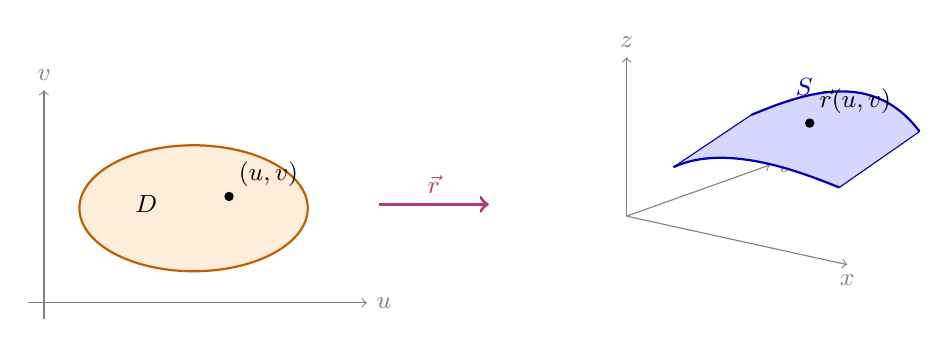
\begin{tikzpicture}[every node/.style={font=\small}]
    \draw[->,gray] (-.2,0)--(4.1,0) node[right] {$u$};
    \draw[->,gray] (0,-.2)--(0,2.7) node[above] {$v$};
    \fill[orange!14] (1.9,1.2) ellipse (1.45 and .8);
    \draw[orange!75!black,thick] (1.9,1.2) ellipse (1.45 and .8);
    \fill (2.35,1.35) circle (1.7pt) node[above right] {$(u,v)$};
    \node at (1.3,1.25) {$D$};
    \draw[->,very thick,magenta!65!black] (4.25,1.25)--(5.65,1.25)
        node[midway,above] {$\vec r$};
    \begin{scope}[shift={(7.4,1.1)},x={(1cm,-.22cm)},y={(.7cm,.25cm)},z={(0cm,.72cm)}]
        \draw[->,gray] (0,0,0)--(2.8,0,0) node[below] {$x$};
        \draw[->,gray] (0,0,0)--(0,2.6,0) node[right] {$y$};
        \draw[->,gray] (0,0,0)--(0,0,2.8) node[above] {$z$};
        \fill[blue!16]
            (.35,.35,.85)..controls(1.1,.25,1.55)and(2,.35,1.25)..(2.35,.5,1.05)
            --(2.25,2.1,1.45)..controls(1.45,2.4,2.2)and(.8,2.1,1.7)..(.25,1.9,1.2)--cycle;
        \draw[blue!70!black,thick]
            (.35,.35,.85)..controls(1.1,.25,1.55)and(2,.35,1.25)..(2.35,.5,1.05);
        \draw[blue!70!black,thick]
            (.25,1.9,1.2)..controls(.8,2.1,1.7)and(1.45,2.4,2.2)..(2.25,2.1,1.45);
        \draw[blue!55!black] (.35,.35,.85)--(.25,1.9,1.2);
        \draw[blue!55!black] (2.35,.5,1.05)--(2.25,2.1,1.45);
        \fill (1.45,1.25,1.65) circle (1.7pt) node[above right] {$\vec r(u,v)$};
        \node[blue!70!black] at (1.1,1.65,2.05) {$S$};
    \end{scope}
\end{tikzpicture}
\end{center}
\endgroup

El dominio $D$ organiza los puntos de $S$. Una cuadrícula en el plano de parámetros se transforma en dos familias de curvas sobre la superficie, lo cual facilita su gráfica y sus cálculos geométricos.

\paragraph{Ejemplo 6. Gráfica de un helicoide}
La parametrización
\[
\vec r(u,v)=\langle u\cos v,u\sin v,v/3\rangle,
\qquad0\leq u\leq2,\quad0\leq v\leq2\pi,
\]
produce una superficie en forma de rampa helicoidal. Para construir su gráfica conviene estudiar por separado el efecto de cada parámetro.

Si se fija $v=v_0$, se obtiene
\[
\vec r(u,v_0)
=\langle u\cos v_0,u\sin v_0,v_0/3\rangle,
\qquad0\leq u\leq2.
\]
Esta curva es un segmento horizontal de longitud $2$, situado a la altura $z=v_0/3$ y dirigido según el ángulo $v_0$ en el plano $xy$. Por ejemplo, $v=0$, $\pi/2$, $\pi$ y $3\pi/2$ producen segmentos que apuntan en cuatro direcciones distintas y se encuentran a alturas diferentes.

Si se fija $u=u_0$, resulta
\[
\vec r(u_0,v)
=\langle u_0\cos v,u_0\sin v,v/3\rangle,
\qquad0\leq v\leq2\pi.
\]
Esta forma es una helice que rodea al eje $z$ con un radio de $u_0$ y que asciende conforme $v$ aumenta. Al dibujar varios segmentos con $v$ fijo y varias hélices con $u$ fijo se forma la cuadrícula del helicoide.

En la figura, la curva naranja corresponde a $v=\pi/2$ y la curva roja a $u=3/2$. La primera muestra un segmento generador y la segunda una hélice completa.

\begingroup\shorthandoff{>}
\begin{center}
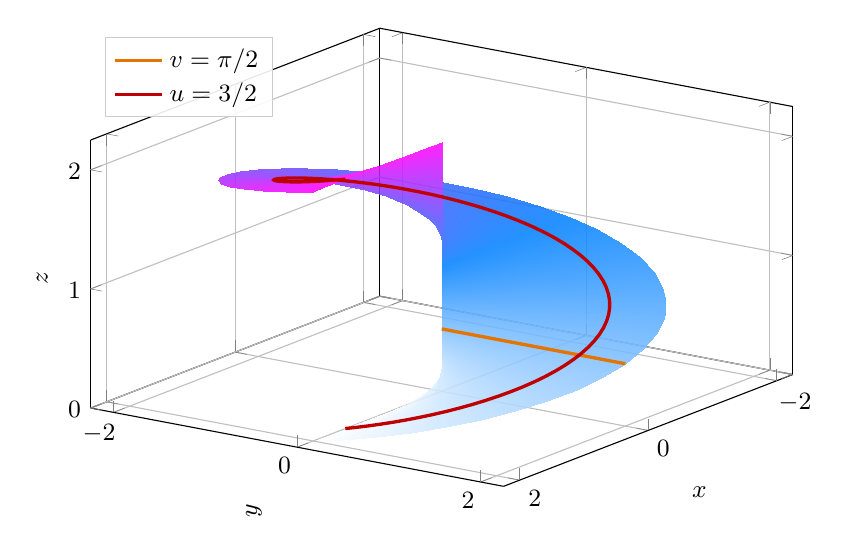
\begin{tikzpicture}
\begin{axis}[width=10.5cm,height=7.4cm,view={125}{27},axis lines=box,
    xlabel={$x$},ylabel={$y$},zlabel={$z$},domain=0:360,y domain=0:2,
    xmin=-2.25,xmax=2.25,ymin=-2.25,ymax=2.25,zmin=0,zmax=2.25,
    xtick={-2,0,2},ytick={-2,0,2},ztick={0,1,2},
    tick label style={font=\small},label style={font=\small},grid=major,
    legend style={font=\small,fill=white,fill opacity=.9,text opacity=1,draw=gray!40,
        at={(.02,.98)},anchor=north west},legend cell align=left,
    samples=41,samples y=13,z buffer=sort]
\addplot3[surf,shader=interp,colormap/cool,opacity=.86,forget plot]
    ({y*cos(x)},{y*sin(x)},{x*pi/540});
\addplot3[orange!90!black,very thick,domain=0:2,samples=25,samples y=0,z buffer=none]
    ({0},{x},{pi/6});
\addlegendentry{$v=\pi/2$}
\addplot3[red!75!black,very thick,domain=0:360,samples=80,samples y=0,z buffer=none]
    ({1.5*cos(x)},{1.5*sin(x)},{x*pi/540});
\addlegendentry{$u=3/2$}
\end{axis}
\end{tikzpicture}
\end{center}
\endgroup

\paragraph{Ejemplo 7. Gráfica de un toro}
Para $R>a>0$,
\[
\vec r(u,v)=\langle(R+a\cos u)\cos v,
(R+a\cos u)\sin v,a\sin u\rangle,
\]
con $0\leq u,v\leq2\pi$, describe un toro. El número $R$ es la distancia del centro del toro al eje $z$ y $a$ es el radio del toro.

Para entender la gráfica, primero se fija $v=v_0$. La curva resultante es
\[
\vec r(u,v_0)=
\langle(R+a\cos u)\cos v_0,
(R+a\cos u)\sin v_0,a\sin u\rangle.
\]
Cuando $u$ recorre $[0,2\pi]$, esta curva forma una circunferencia de radio $a$ en un plano vertical que contiene al eje $z$ desplazada radialmente a una distancia $R$ del eje.

Si se fija $u=u_0$, se obtiene
\[
\vec r(u_0,v)=
\langle(R+a\cos u_0)\cos v,
(R+a\cos u_0)\sin v,a\sin u_0\rangle.
\]
Esta es una circunferencia horizontal: su radio es $R+a\cos u_0$ y su altura es $a\sin u_0$. Al variar $u_0$, estas circunferencias horizontales cubren el toro.

La curva naranja es la circunferencia generatriz $v=0$ y la curva roja es la circunferencia horizontal $u=\pi/3$.

\begingroup\shorthandoff{>}
\begin{center}
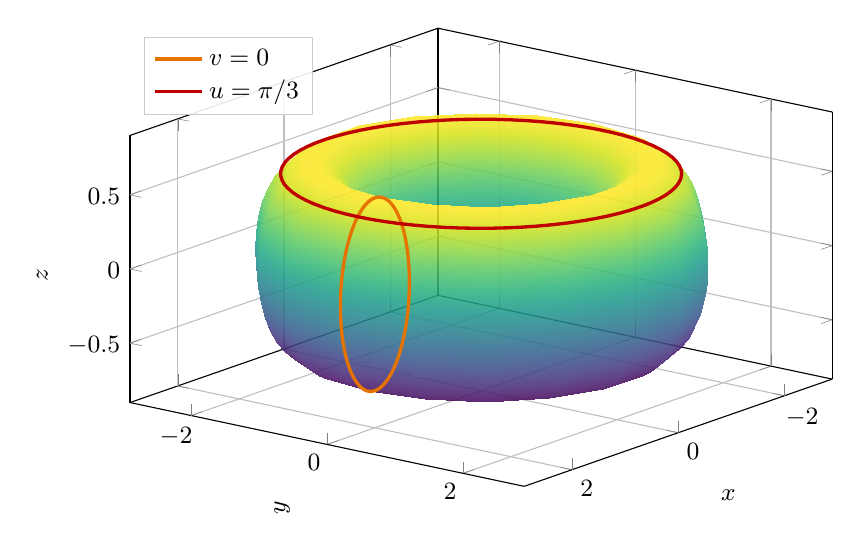
\begin{tikzpicture}
\begin{axis}[width=10.5cm,height=7.4cm,view={128}{27},axis lines=box,
    xlabel={$x$},ylabel={$y$},zlabel={$z$},domain=0:360,y domain=0:360,
    xmin=-2.9,xmax=2.9,ymin=-2.9,ymax=2.9,zmin=-.9,zmax=.9,
    xtick={-2,0,2},ytick={-2,0,2},ztick={-.5,0,.5},
    tick label style={font=\small},label style={font=\small},grid=major,
    legend style={font=\small,fill=white,fill opacity=.9,text opacity=1,draw=gray!40,
        at={(.02,.98)},anchor=north west},legend cell align=left,
    samples=37,samples y=19,z buffer=sort]
\addplot3[surf,shader=interp,colormap/viridis,opacity=.86,forget plot]
    ({(2+.65*cos(x))*cos(y)},{(2+.65*cos(x))*sin(y)},{.65*sin(x)});
\addplot3[orange!90!black,very thick,domain=0:360,samples=80,samples y=0,z buffer=none]
    ({2+.65*cos(x)},{0},{.65*sin(x)});
\addlegendentry{$v=0$}
\addplot3[red!75!black,very thick,domain=0:360,samples=80,samples y=0,z buffer=none]
    ({(2+.65*cos(60))*cos(x)},{(2+.65*cos(60))*sin(x)},{.65*sin(60)});
\addlegendentry{$u=\pi/3$}
\end{axis}
\end{tikzpicture}
\end{center}
\endgroup

\subsubsection{Cómo construir una parametrización}

\paragraph{Superficies de la forma $z=f(x,y)$}
Los valores de $x$ y $y$ pueden emplearse como parámetros:
\[
x=u,\qquad y=v,\qquad z=f(u,v).
\]
Por tanto,
\[
\vec r(u,v)=\langle u,v,f(u,v)\rangle,
\qquad (u,v)\in R.
\]
La elección también puede adaptarse al dominio. Si $R$ es circular, suele resultar conveniente usar $x=u\cos v$, $y=u\sin v$.

La figura muestra la gráfica $z=u^2+v^2$ sobre $R=[-1,1]^2$. En este caso el dominio es un cuadrado y los parámetros $u$ y $v$ coinciden con las coordenadas $x$ y $y$.

\begingroup\shorthandoff{>}
\begin{center}
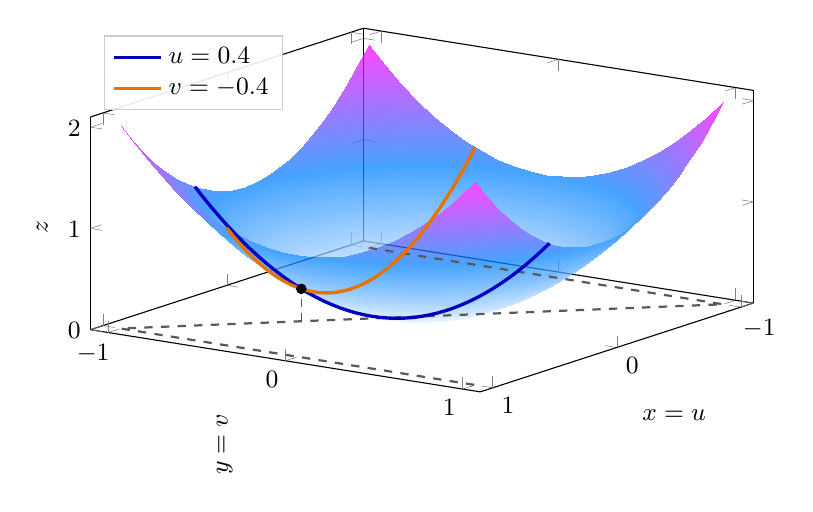
\begin{tikzpicture}
\begin{axis}[width=10cm,height=6.2cm,view={125}{27},axis lines=box,
    xlabel={$x=u$},ylabel={$y=v$},zlabel={$z$},
    xmin=-1.1,xmax=1.1,ymin=-1.1,ymax=1.1,zmin=0,zmax=2.1,
    xtick={-1,0,1},ytick={-1,0,1},ztick={0,1,2},
    tick label style={font=\small},label style={font=\small},
    domain=-1:1,y domain=-1:1,samples=23,samples y=23,z buffer=sort,
    legend style={font=\small,fill=white,fill opacity=.9,text opacity=1,
        draw=gray!40,at={(.02,.98)},anchor=north west},
    legend cell align=left]
\addplot3[surf,shader=interp,colormap/cool,opacity=.72,forget plot]
    {x^2+y^2};
\addplot3[gray!70!black,dashed,thick,forget plot]
    coordinates {(-1,-1,0) (1,-1,0) (1,1,0) (-1,1,0) (-1,-1,0)};
\addplot3[gray!70!black,densely dashed,forget plot]
    coordinates {(.4,-.4,0) (.4,-.4,.32)};
\addplot3[blue!75!black,very thick,domain=-1:1,samples=45,
    samples y=0,z buffer=none]
    ({.4},{x},{.16+x^2});
\addlegendentry{$u=0.4$}
\addplot3[orange!90!black,very thick,domain=-1:1,samples=45,
    samples y=0,z buffer=none]
    ({x},{-.4},{x^2+.16});
\addlegendentry{$v=-0.4$}
\addplot3[only marks,mark=*,mark size=1.7pt,black,forget plot]
    coordinates {(.4,-.4,.32)};
\end{axis}
\end{tikzpicture}
\end{center}
\endgroup

\paragraph{Superficies de revolución}
Sea $\rho=g(z)\geq0$ el radio de un perfil en el plano $\rho z$. Al girarlo alrededor del eje $z$ se obtiene
\[
\vec r(u,v)=\langle g(u)\cos v,g(u)\sin v,u\rangle,
\qquad0\leq v\leq2\pi.
\]
Al fijar $u=u_0$, el ángulo $v$ recorre una circunferencia horizontal de radio $g(u_0)$ a la altura $z=u_0$. Por ejemplo, el perfil $g(u)=1-u/2$, $0\leq u\leq2$, genera la superficie lateral de un cono.

\begingroup\shorthandoff{>}
\begin{center}
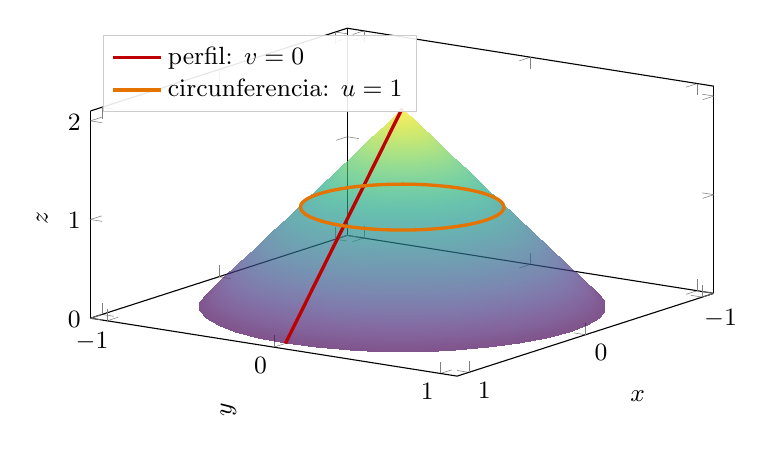
\begin{tikzpicture}
\begin{axis}[width=9.5cm,height=6cm,view={125}{26},axis lines=box,
    xlabel={$x$},ylabel={$y$},zlabel={$z$},
    xmin=-1.1,xmax=1.1,ymin=-1.1,ymax=1.1,zmin=0,zmax=2.1,
    xtick={-1,0,1},ytick={-1,0,1},ztick={0,1,2},
    tick label style={font=\small},label style={font=\small},
    domain=0:360,y domain=0:2,samples=37,samples y=13,z buffer=sort,
    legend style={font=\small,fill=white,fill opacity=.9,text opacity=1,
        draw=gray!40,at={(.02,.98)},anchor=north west},
    legend cell align=left]
\addplot3[surf,shader=interp,colormap/viridis,opacity=.68,forget plot]
    ({(1-y/2)*cos(x)},{(1-y/2)*sin(x)},{y});
\addplot3[red!75!black,very thick,domain=0:2,samples=35,
    samples y=0,z buffer=none]
    ({1-x/2},{0},{x});
\addlegendentry{perfil: $v=0$}
\addplot3[orange!90!black,very thick,domain=0:360,samples=80,
    samples y=0,z buffer=none]
    ({.5*cos(x)},{.5*sin(x)},{1});
\addlegendentry{circunferencia: $u=1$}
\end{axis}
\end{tikzpicture}
\end{center}
\endgroup

De forma equivalente, si una curva del plano $xz$ se escribe como $(x,z)=(p(u),q(u))$, su rotación alrededor del eje $z$ es
\[
\vec r(u,v)=\langle p(u)\cos v,p(u)\sin v,q(u)\rangle.
\]
Para girar la gráfica $y=g(x)$ alrededor del eje $x$ se usa
\[
\vec r(u,v)=\langle u,g(u)\cos v,g(u)\sin v\rangle.
\]
En este caso, al fijar $u=u_0$ se obtiene una circunferencia en el plano $x=u_0$.

\begingroup\shorthandoff{>}
\begin{center}
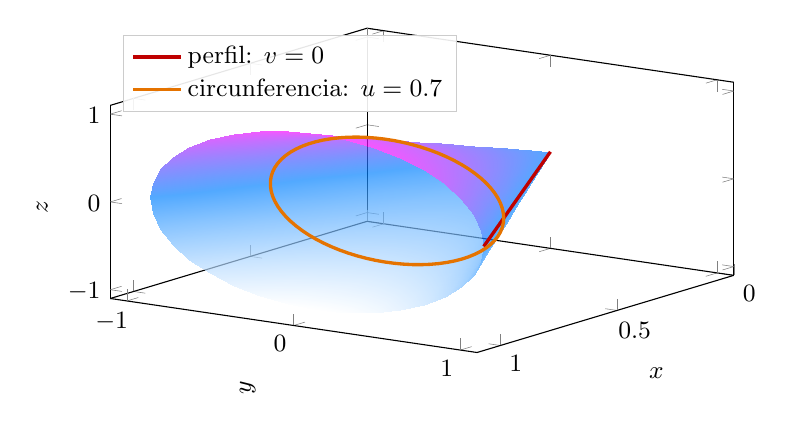
\begin{tikzpicture}
\begin{axis}[width=9.5cm,height=5.7cm,view={125}{26},axis lines=box,
    xlabel={$x$},ylabel={$y$},zlabel={$z$},
    xmin=0,xmax=1.1,ymin=-1.1,ymax=1.1,zmin=-1.1,zmax=1.1,
    xtick={0,.5,1},ytick={-1,0,1},ztick={-1,0,1},
    tick label style={font=\small},label style={font=\small},
    domain=0:360,y domain=0:1,samples=37,samples y=13,z buffer=sort,
    legend style={font=\small,fill=white,fill opacity=.9,text opacity=1,
        draw=gray!40,at={(.02,.98)},anchor=north west},
    legend cell align=left]
\addplot3[surf,shader=interp,colormap/cool,opacity=.68,forget plot]
    ({y},{y*cos(x)},{y*sin(x)});
\addplot3[red!75!black,very thick,domain=0:1,samples=35,
    samples y=0,z buffer=none]
    ({x},{x},{0});
\addlegendentry{perfil: $v=0$}
\addplot3[orange!90!black,very thick,domain=0:360,samples=80,
    samples y=0,z buffer=none]
    ({.7},{.7*cos(x)},{.7*sin(x)});
\addlegendentry{circunferencia: $u=0.7$}
\end{axis}
\end{tikzpicture}
\end{center}
\endgroup

\paragraph{Ejemplo 8. Parametrización de un paraboloide}
Para $S:z=x^2+y^2$, $0\leq z\leq4$, una parametrización cartesiana es
\[
\vec r(u,v)=\langle u,v,u^2+v^2\rangle,
\qquad u^2+v^2\leq4.
\]
Una forma polar que usa un dominio rectangular es
\[
\vec r(\rho,\theta)
=\langle\rho\cos\theta,\rho\sin\theta,\rho^2\rangle,
\qquad0\leq\rho\leq2,\quad0\leq\theta\leq2\pi.
\]
La figura muestra la porción de paraboloide descrita por ambas parametrizaciones.

\begingroup\shorthandoff{>}
\begin{center}
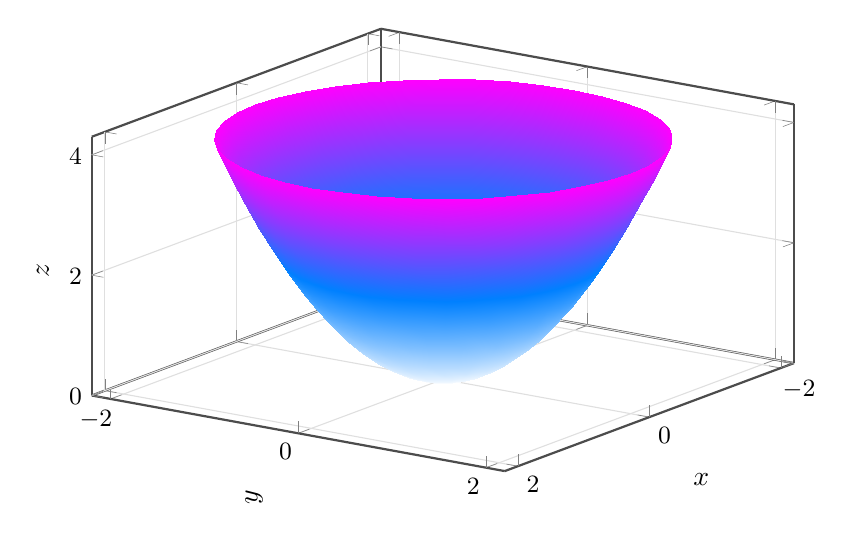
\begin{tikzpicture}
\begin{axis}[width=10.5cm,height=7.2cm,view={125}{27},axis lines=box,
    axis line style={black!70,thick},
    xlabel={$x$},ylabel={$y$},zlabel={$z$},
    xmin=-2.2,xmax=2.2,ymin=-2.2,ymax=2.2,zmin=0,zmax=4.3,
    xtick={-2,0,2},ytick={-2,0,2},ztick={0,2,4},
    tick label style={font=\small},label style={font=\normalsize},
    grid=major,grid style={gray!25},domain=0:360,y domain=0:2,
    samples=41,samples y=17,z buffer=sort]
\addplot3[surf,shader=interp,colormap/cool]
    ({y*cos(x)},{y*sin(x)},{y^2});
\end{axis}
\end{tikzpicture}
\end{center}
\endgroup

\paragraph{Ejemplo 9. Parametrización de un cono por revolución}
El segmento del plano $\rho z$ dado por $\rho=u$, $z=h(1-u/a)$, $0\leq u\leq a$, gira alrededor del eje $z$. La superficie lateral del cono queda parametrizada por
\[
\vec r(u,v)=\left\langle u\cos v,u\sin v,
h\left(1-\frac ua\right)\right\rangle,
\qquad0\leq u\leq a,\quad0\leq v\leq2\pi.
\]
La figura muestra el caso $a=1$ y $h=1.5$.

\begingroup\shorthandoff{>}
\begin{center}
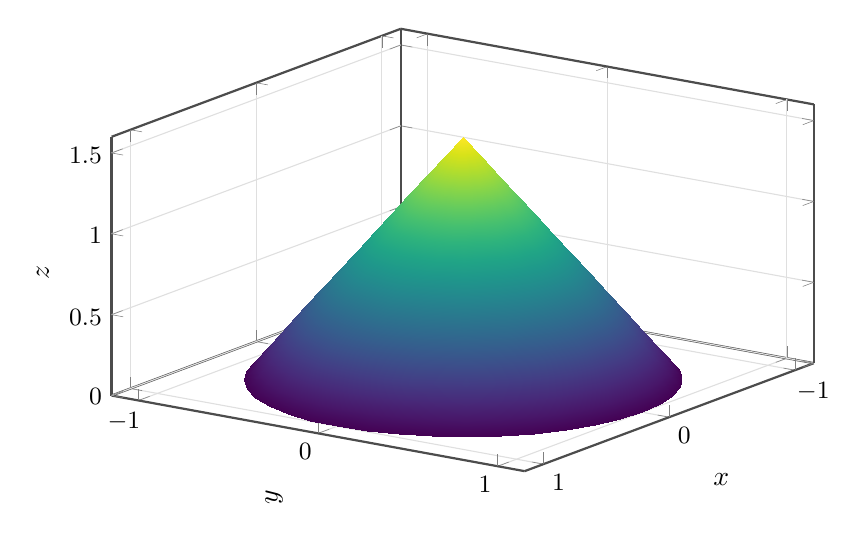
\begin{tikzpicture}
\begin{axis}[width=10.5cm,height=7.2cm,view={125}{27},axis lines=box,
    axis line style={black!70,thick},
    xlabel={$x$},ylabel={$y$},zlabel={$z$},
    xmin=-1.15,xmax=1.15,ymin=-1.15,ymax=1.15,zmin=0,zmax=1.6,
    xtick={-1,0,1},ytick={-1,0,1},ztick={0,.5,1,1.5},
    tick label style={font=\small},label style={font=\normalsize},
    grid=major,grid style={gray!25},domain=0:360,y domain=0:1,
    samples=41,samples y=13,z buffer=sort]
\addplot3[surf,shader=interp,colormap/viridis]
    ({y*cos(x)},{y*sin(x)},{1.5*(1-y)});
\end{axis}
\end{tikzpicture}
\end{center}
\endgroup

\paragraph{Ejemplo 10. Parametrización de una esfera}
El semicírculo de radio $a$ en el plano $\rho z$ puede escribirse como $\rho=a\sin\varphi$, $z=a\cos\varphi$. Al girarlo alrededor del eje $z$ se obtiene
\[
\vec r(\varphi,\theta)=
\langle a\sin\varphi\cos\theta,
a\sin\varphi\sin\theta,a\cos\varphi\rangle,
\]
donde $0\leq\varphi\leq\pi$ y $0\leq\theta\leq2\pi$.
La figura muestra el caso $a=1$.

\begingroup\shorthandoff{>}
\begin{center}
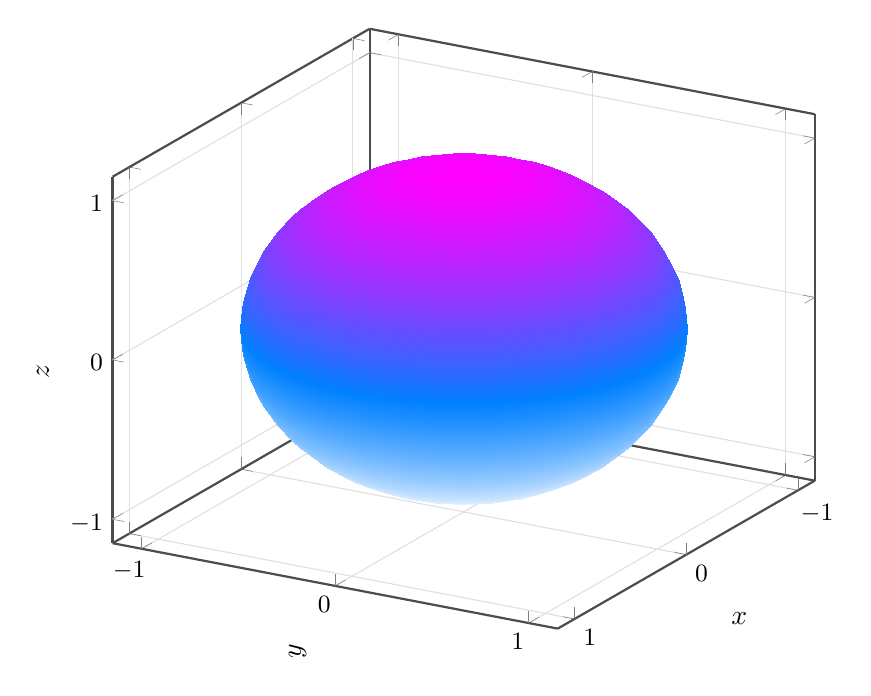
\begin{tikzpicture}
\begin{axis}[width=10.5cm,height=9.2cm,view={120}{25},axis lines=box,
    axis line style={black!70,thick},
    xlabel={$x$},ylabel={$y$},zlabel={$z$},
    xmin=-1.15,xmax=1.15,ymin=-1.15,ymax=1.15,zmin=-1.15,zmax=1.15,
    xtick={-1,0,1},ytick={-1,0,1},ztick={-1,0,1},
    tick label style={font=\small},label style={font=\normalsize},
    grid=major,grid style={gray!25},domain=0:360,y domain=0:180,
    samples=49,samples y=25,z buffer=sort]
\addplot3[surf,shader=interp,colormap/cool]
    ({sin(y)*cos(x)},{sin(y)*sin(x)},{cos(y)});
\end{axis}
\end{tikzpicture}
\end{center}
\endgroup

\newpage
\subsubsection{Vector normal y plano tangente}

Sea $\vec r(u,v)$ una parametrización con derivadas parciales continuas cerca de un punto interior $(u_0,v_0)$ de su dominio, y sea $P_0=\vec r(u_0,v_0)$. Al fijar $v=v_0$ y variar $u$ se obtiene una curva sobre la superficie, al fijar $u=u_0$ y variar $v$ se obtiene otra. Ambas pasan por $P_0$, y sus vectores tangentes en ese punto son
\[
\vec r_u(u_0,v_0)=\frac{\partial\vec r}{\partial u}(u_0,v_0),
\qquad
\vec r_v(u_0,v_0)=\frac{\partial\vec r}{\partial v}(u_0,v_0).
\]
Para incrementos pequeños $\Delta u$ y $\Delta v$, la aproximación lineal es
\[
\vec r(u_0+\Delta u,v_0+\Delta v)
\approx \vec r(u_0,v_0)
+\vec r_u(u_0,v_0)\Delta u
+\vec r_v(u_0,v_0)\Delta v.
\]
Así, cerca de $P_0$ la superficie se aproxima por el plano generado por los dos vectores tangentes:
\[
\langle x,y,z\rangle
=\vec r(u_0,v_0)+s\vec r_u(u_0,v_0)+t\vec r_v(u_0,v_0),
\qquad s,t\in\mathbb R.
\]

\begin{mydefinition}{Superficie paramétrica regular}
Una parametrización $\vec r(u,v)$ es regular en $(u,v)$ si
\[
\vec r_u(u,v)\times\vec r_v(u,v)\neq\mathbf0.
\]
En tal punto existen dos direcciones tangentes independientes y un plano tangente bien definido.
\end{mydefinition}

En un punto regular, el producto cruz
\[
\mathbf{N}_0=\vec r_u(u_0,v_0)\times\vec r_v(u_0,v_0)
\]
es distinto de cero y perpendicular a los dos vectores tangentes. Por ello, si $P_0=(x_0,y_0,z_0)$, un punto $(x,y,z)$ pertenece al plano tangente precisamente cuando su desplazamiento desde $P_0$ es perpendicular a $\mathbf{N}_0$:
\[
\mathbf{N}_0\cdot\langle x-x_0,y-y_0,z-z_0\rangle=0.
\]
Dividir $\mathbf{N}_0$ entre su norma produce la normal unitaria
\[
\mathbf{n}=\frac{\vec r_u\times\vec r_v}
{\lVert\vec r_u\times\vec r_v\rVert}.
\]
La elección del orden de los parámetros fija su sentido: $\vec r_v\times\vec r_u=-\vec r_u\times\vec r_v$ da la normal unitaria opuesta, pero el mismo plano tangente.

En la figura, las curvas naranja y magenta son las imágenes de las rectas $v=v_0$ y $u=u_0$ del dominio. Sus tangentes generan el plano gris en $P_0$, mientras que la flecha roja representa una normal perpendicular a ese plano.

\begingroup
\shorthandoff{>}
\begin{center}
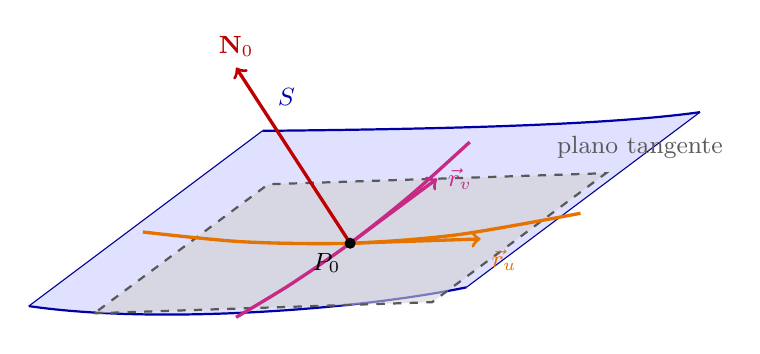
\begin{tikzpicture}[x={(1.95cm,-.41cm)},y={(1.38cm,.55cm)},z={(0cm,1.58cm)},
    every node/.style={font=\small}]
    \fill[blue!12]
        (.25,.2,1.01)..controls(1.1,.15,1.1)and(2.4,.15,1.55)..(3.1,.2,1.9)
        --(3.1,2.35,2.56)..controls(2.35,2.5,2.2)and(1.1,2.5,1.85)..(.25,2.35,1.67)--cycle;
    \draw[blue!65!black,thick]
        (.25,.2,1.01)..controls(1.1,.15,1.1)and(2.4,.15,1.55)..(3.1,.2,1.9);
    \draw[blue!65!black,thick]
        (.25,2.35,1.67)..controls(1.1,2.5,1.85)and(2.35,2.5,2.2)..(3.1,2.35,2.56);
    \draw[blue!55!black] (.25,.2,1.01)--(.25,2.35,1.67);
    \draw[blue!55!black] (3.1,.2,1.9)--(3.1,2.35,2.56);
    \fill[gray!35,opacity=.58]
        (.5,.45,.93)--(2.7,.45,1.59)--(2.7,2.05,2.07)--(.5,2.05,1.41)--cycle;
    \draw[gray!70!black,dashed,thick]
        (.5,.45,.93)--(2.7,.45,1.59)--(2.7,2.05,2.07)--(.5,2.05,1.41)--cycle;
    \draw[orange!90!black,very thick]
        plot[smooth] coordinates {(.25,1.25,1.24) (.9,1.25,1.33)
            (1.6,1.25,1.5) (2.3,1.25,1.75) (3.1,1.25,2.13)};
    \draw[magenta!80!black,very thick]
        plot[smooth] coordinates {(1.6,.2,1.27) (1.6,.7,1.36)
            (1.6,1.25,1.5) (1.6,1.8,1.69) (1.6,2.35,1.93)};
    \coordinate (P) at (1.6,1.25,1.5);
    \draw[->,orange!90!black,very thick] (P)--++(.85,0,.255)
        node[below right] {$\vec r_u$};
    \draw[->,magenta!80!black,very thick] (P)--++(0,.8,.24)
        node[right] {$\vec r_v$};
    \draw[->,red!75!black,very thick] (P)--++(-.435,-.435,1.45)
        node[above] {$\mathbf{N}_0$};
    \fill (P) circle (2pt) node[below left] {$P_0$};
    \node[blue!70!black] at (.3,2.5,1.9) {$S$};
    \node[gray!70!black] at (2.9,2.08,2.32) {plano tangente};
\end{tikzpicture}
\end{center}
\endgroup

Para una gráfica $\vec r(u,v)=\langle u,v,f(u,v)\rangle$, los vectores tangentes son $\vec r_u=\langle1,0,f_u\rangle$ y $\vec r_v=\langle0,1,f_v\rangle$. En consecuencia, $\mathbf{N}=\langle-f_u,-f_v,1\rangle$ y la ecuación anterior se reduce a
\[
z-z_0=f_u(u_0,v_0)(x-u_0)+f_v(u_0,v_0)(y-v_0),
\qquad z_0=f(u_0,v_0).
\]

\subsubsection{Área de una superficie paramétrica}

Sea $(u_0,v_0)$ un punto interior del dominio $D$. Un rectángulo pequeño con lados $\Delta u$ y $\Delta v$ se transforma en un parche curvo de la superficie. Cerca de $P_0=\vec r(u_0,v_0)$, los desplazamientos a lo largo de sus lados se aproximan por $\vec r_u(u_0,v_0)\Delta u$ y $\vec r_v(u_0,v_0)\Delta v$. Estos vectores forman un paralelogramo tangente, como muestra la figura.

\begingroup\shorthandoff{>}
\begin{center}
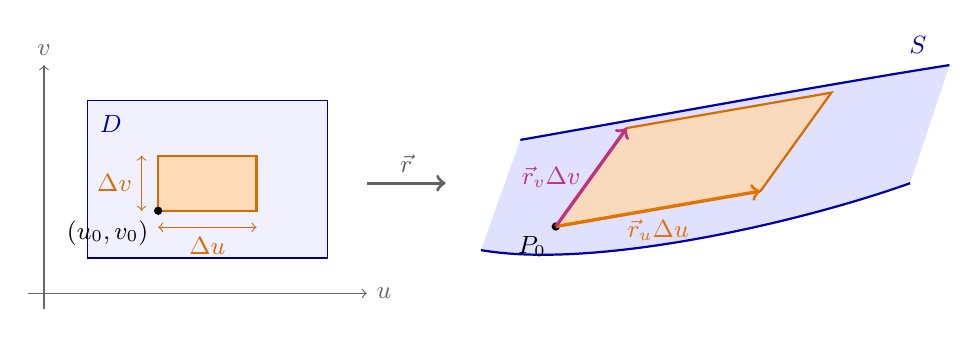
\begin{tikzpicture}[every node/.style={font=\small}]
    \draw[->,gray!80!black] (-.2,0)--(4.1,0) node[right] {$u$};
    \draw[->,gray!80!black] (0,-.2)--(0,2.9) node[above] {$v$};
    \fill[blue!6] (.55,.45) rectangle (3.6,2.45);
    \draw[blue!60!black] (.55,.45) rectangle (3.6,2.45);
    \node[blue!65!black] at (.85,2.15) {$D$};
    \fill[orange!28] (1.45,1.05) rectangle (2.7,1.75);
    \draw[orange!85!black,thick] (1.45,1.05) rectangle (2.7,1.75);
    \fill (1.45,1.05) circle (1.5pt) node[below left] {$(u_0,v_0)$};
    \draw[<->,orange!85!black] (1.45,.84)--(2.7,.84)
        node[midway,below] {$\Delta u$};
    \draw[<->,orange!85!black] (1.24,1.05)--(1.24,1.75)
        node[midway,left] {$\Delta v$};
    \draw[->,very thick,gray!75!black] (4.1,1.4)--(5.1,1.4)
        node[midway,above] {$\vec r$};
    \fill[blue!12]
        (5.55,.55)..controls(7,.3)and(9.6,.9)..(11,1.4)
        --(11.5,2.9)..controls(9.9,2.65)and(7.2,2.15)..(6.05,1.95)--cycle;
    \draw[blue!65!black,thick]
        (5.55,.55)..controls(7,.3)and(9.6,.9)..(11,1.4);
    \draw[blue!65!black,thick]
        (6.05,1.95)..controls(7.2,2.15)and(9.9,2.65)..(11.5,2.9);
    \node[blue!65!black] at (11.1,3.15) {$S$};
    \fill[orange!30,opacity=.85]
        (6.5,.85)--(9.1,1.3)--(10,2.55)--(7.4,2.1)--cycle;
    \draw[orange!85!black,thick]
        (6.5,.85)--(9.1,1.3)--(10,2.55)--(7.4,2.1)--cycle;
    \fill (6.5,.85) circle (1.5pt) node[below left] {$P_0$};
    \draw[->,orange!90!black,very thick] (6.5,.85)--(9.1,1.3)
        node[midway,below] {$\vec r_u\Delta u$};
    \draw[->,magenta!75!black,very thick] (6.5,.85)--(7.4,2.1)
        node[midway,left] {$\vec r_v\Delta v$};
\end{tikzpicture}
\end{center}
\endgroup

El área del paralelogramo es la norma del producto cruz de sus lados. Por ello, el área $\Delta S$ del parche curvo satisface aproximadamente
\[
\Delta S\approx
\lVert\vec r_u\times\vec r_v\rVert\,\Delta u\,\Delta v.
\]
Al sumar estas aproximaciones y refinar la partición de $D$, se obtiene el siguiente resultado.

\begin{mytheorem}{Área de una superficie paramétrica}
Sea $\vec r:D\to\mathbb R^3$ una parametrización regular, suave y uno a uno en el interior de $D$. Entonces
\[
\operatorname{area}(S)
=\iint_D\lVert\vec r_u\times\vec r_v\rVert\,du\,dv.
\]
El diferencial de superficie es
\[
dS=\lVert\vec r_u\times\vec r_v\rVert\,du\,dv.
\]
\end{mytheorem}

Para una gráfica $\vec r(u,v)=\langle u,v,f(u,v)\rangle$,
\[
\vec r_u\times\vec r_v
=\langle-f_u,-f_v,1\rangle,
\]
de modo que la fórmula paramétrica recupera
$dS=\sqrt{1+f_u^2+f_v^2}\,du\,dv$.

\paragraph{Ejemplo 11. Plano: normal, plano tangente y área}
Considérese
\[
\vec r(u,v)=\langle u,v,1+2u-v\rangle,
\qquad0\leq u\leq1,\quad0\leq v\leq2.
\]
Se tiene
\[
\vec r_u=\langle1,0,2\rangle,
\qquad
\vec r_v=\langle0,1,-1\rangle,
\qquad
\vec r_u\times\vec r_v=\langle-2,1,1\rangle.
\]
En $P_0=\vec r(0,0)=(0,0,1)$, el plano tangente es
\[
-2x+y+(z-1)=0.
\]
Como la norma del vector normal es $\sqrt6$, el área del parche es
\[
\int_0^1\int_0^2\sqrt6\,dv\,du=2\sqrt6.
\]
La figura muestra el parche sobre el rectángulo de parámetros. La flecha roja representa la dirección normal $\langle-2,1,1\rangle$; como el plano tiene la misma inclinación en todos sus puntos, el factor de área $\sqrt6$ es constante.

\begingroup\shorthandoff{>}
\begin{center}
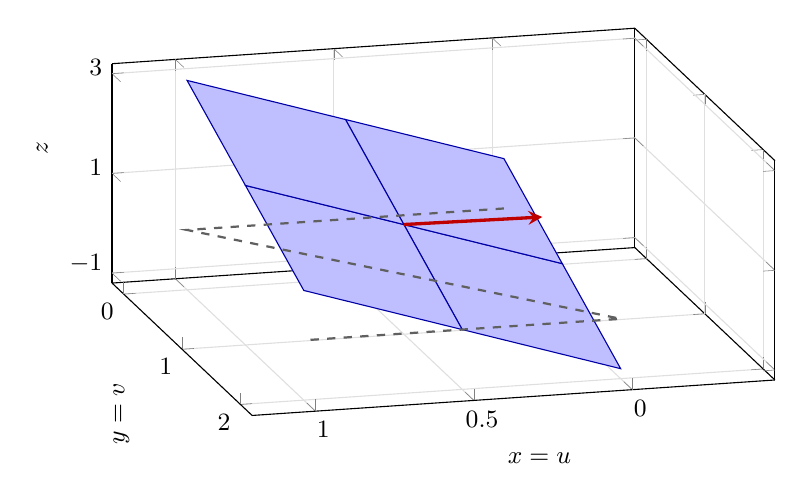
\begin{tikzpicture}
\begin{axis}[width=10cm,height=6.5cm,view={165}{32},axis lines=box,
    xlabel={$x=u$},ylabel={$y=v$},zlabel={$z$},
    xmin=-.45,xmax=1.2,ymin=-.2,ymax=2.2,zmin=-1.2,zmax=3.2,
    xtick={0,.5,1},ytick={0,1,2},ztick={-1,1,3},
    tick label style={font=\small},label style={font=\small},
    grid=major,grid style={gray!25},domain=0:1,y domain=0:2,
    samples=3,samples y=3,z buffer=sort]
\addplot3[surf,shader=flat,draw=blue!65!black,fill=blue!25]
    {1+2*x-y};
\addplot3[gray!75!black,dashed,thick]
    coordinates {(0,0,0) (1,0,0) (1,2,0) (0,2,0) (0,0,0)};
\addplot3[red!75!black,very thick,-stealth]
    coordinates {(.5,1,1) (.1,1.2,1.2)};
\end{axis}
\end{tikzpicture}
\end{center}
\endgroup

\paragraph{Ejemplo 12. Paraboloide hiperbólico}
Sea
\[
\vec r(u,v)=\langle u,v,u^2-v^2\rangle,
\qquad D=\{(u,v):u^2+v^2\leq1\}.
\]
Entonces
\[
\vec r_u\times\vec r_v=\langle-2u,2v,1\rangle.
\]
En $(u,v)=(1/2,1/2)$, el punto es $P_0=(1/2,1/2,0)$ y puede tomarse $\mathbf{N}_0=\langle-1,1,1\rangle$. El plano tangente queda
\[
-(x-1/2)+(y-1/2)+z=0,
\qquad\text{es decir,}\qquad -x+y+z=0.
\]
Además,
\begin{align*}
\operatorname{area}(S)
&=\iint_D\sqrt{1+4u^2+4v^2}\,du\,dv\\
&=\int_0^{2\pi}\int_0^1\sqrt{1+4\rho^2}\,\rho\,d\rho\,d\theta
=\frac{\pi}{6}(5\sqrt5-1).
\end{align*}
\begingroup\shorthandoff{>}
\begin{center}
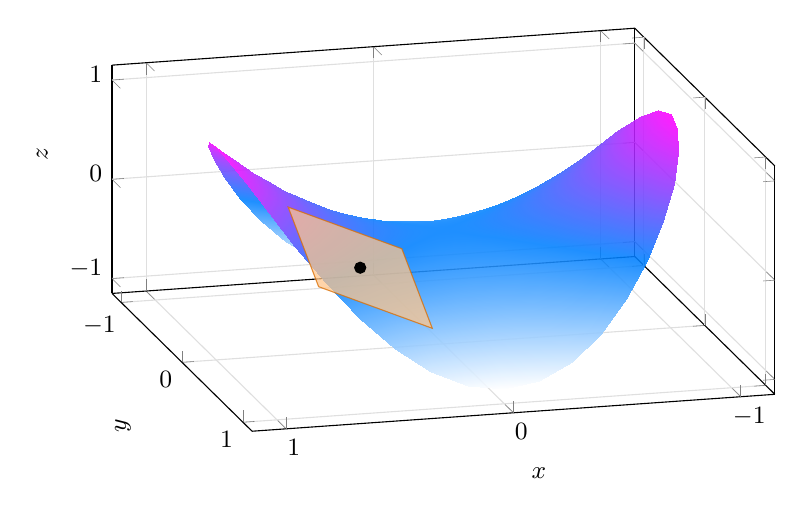
\begin{tikzpicture}
\begin{axis}[width=10cm,height=6.7cm,view={165}{32},axis lines=box,
    xlabel={$x$},ylabel={$y$},zlabel={$z$},
    xmin=-1.15,xmax=1.15,ymin=-1.15,ymax=1.15,zmin=-1.15,zmax=1.15,
    xtick={-1,0,1},ytick={-1,0,1},ztick={-1,0,1},
    tick label style={font=\small},label style={font=\small},
    grid=major,grid style={gray!25},domain=0:360,y domain=0:1,
    samples=41,samples y=17,z buffer=sort]
\addplot3[surf,shader=interp,colormap/cool,opacity=.88]
    ({y*cos(x)},{y*sin(x)},{y^2*(cos(x)^2-sin(x)^2)});
\addplot3[surf,shader=flat,draw=orange!85!black,fill=orange!45,
    opacity=.75,domain=.25:.75,y domain=.25:.75,
    samples=2,samples y=2,z buffer=none]
    {x-y};
\addplot3[only marks,mark=*,mark size=2pt,black]
    coordinates {(.5,.5,0)};
\end{axis}
\end{tikzpicture}
\end{center}
\endgroup
El disco $D$ recorta la superficie con una frontera circular. En la figura, el pequeño parche naranja pertenece al plano tangente $z=x-y$ en $P_0$; su inclinación aproxima la superficie cerca de ese punto.

\paragraph{Ejemplo 13. Superficie lateral de un cilindro}
Para un cilindro de radio $a$ y altura $L$ se usa
\[
\vec r(u,v)=\langle a\cos u,a\sin u,v\rangle,
\qquad0\leq u\leq2\pi,\quad0\leq v\leq L.
\]
Sus vectores fundamentales son
\begin{align*}
\vec r_u&=\langle-a\sin u,a\cos u,0\rangle,\\
\vec r_v&=\langle0,0,1\rangle,\\
\vec r_u\times\vec r_v&=\langle a\cos u,a\sin u,0\rangle.
\end{align*}
Este último apunta hacia afuera y tiene norma $a$. Por tanto,
\[
\operatorname{area}(S)=\int_0^{2\pi}\int_0^L a\,dv\,du=2\pi aL.
\]
En el punto $(a,0,v_0)$, el plano tangente es $x=a$.
La figura representa $a=1$ y $L=2$. La curva naranja es una sección horizontal y la flecha roja señala la normal exterior en $(1,0,1)$; su dirección es radial, mientras que su norma permanece igual a $a$ en todo el cilindro.

\begingroup\shorthandoff{>}
\begin{center}
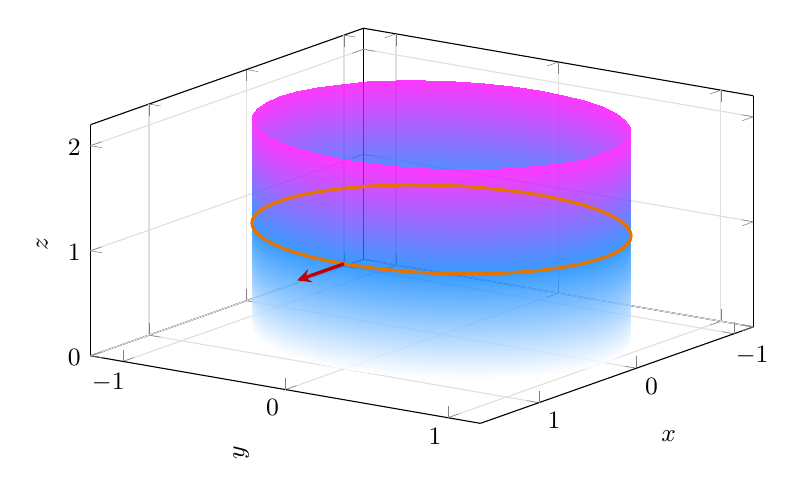
\begin{tikzpicture}
\begin{axis}[width=10cm,height=6.6cm,view={125}{27},axis lines=box,
    xlabel={$x$},ylabel={$y$},zlabel={$z$},
    xmin=-1.2,xmax=1.6,ymin=-1.2,ymax=1.2,zmin=0,zmax=2.2,
    xtick={-1,0,1},ytick={-1,0,1},ztick={0,1,2},
    tick label style={font=\small},label style={font=\small},
    grid=major,grid style={gray!25},domain=0:360,y domain=0:2,
    samples=41,samples y=13,z buffer=sort]
\addplot3[surf,shader=interp,colormap/cool,opacity=.78]
    ({cos(x)},{sin(x)},{y});
\addplot3[orange!90!black,very thick,domain=0:360,
    samples=85,samples y=0,z buffer=none]
    ({cos(x)},{sin(x)},{1});
\addplot3[red!75!black,very thick,-stealth]
    coordinates {(1,0,1) (1.48,0,1)};
\end{axis}
\end{tikzpicture}
\end{center}
\endgroup

\newpage
\paragraph{Ejemplo 14. Esfera paramétrica}
Para la esfera de radio $a$, considérese la parametrización del Ejemplo 10. El producto cruz es
\[
\vec r_\varphi\times\vec r_\theta
=a^2\sin\varphi
\langle\sin\varphi\cos\theta,
\sin\varphi\sin\theta,\cos\varphi\rangle.
\]
Cuando $0<\varphi<\pi$, apunta hacia afuera y tiene norma $a^2\sin\varphi$. En consecuencia,
\[
\operatorname{area}(S)
=\int_0^{2\pi}\int_0^\pi a^2\sin\varphi\,d\varphi\,d\theta
=4\pi a^2.
\]
La parametrización deja de ser regular en los polos, donde $\sin\varphi=0$, pero esos puntos no modifican el valor de la integral de área.
En $(a,0,0)$, correspondiente a $(\varphi,\theta)=(\pi/2,0)$, el vector normal es paralelo a $\langle1,0,0\rangle$ y el plano tangente es $x=a$.
Para $a=1$, la figura muestra ese plano tangente como un parche gris y la normal exterior como una flecha roja. La normal cambia de dirección sobre la esfera, aunque su longitud antes de normalizar depende solo de $\varphi$.

\begingroup\shorthandoff{>}
\begin{center}
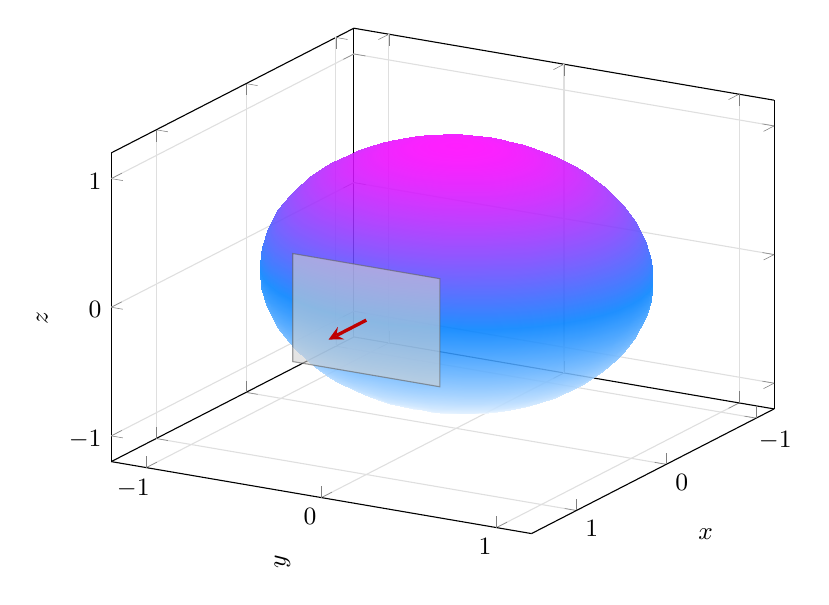
\begin{tikzpicture}
\begin{axis}[width=10cm,height=8cm,view={120}{25},axis lines=box,
    xlabel={$x$},ylabel={$y$},zlabel={$z$},
    xmin=-1.2,xmax=1.5,ymin=-1.2,ymax=1.2,zmin=-1.2,zmax=1.2,
    xtick={-1,0,1},ytick={-1,0,1},ztick={-1,0,1},
    tick label style={font=\small},label style={font=\small},
    grid=major,grid style={gray!25},domain=0:360,y domain=0:180,
    samples=49,samples y=25,z buffer=sort]
\addplot3[surf,shader=interp,colormap/cool,opacity=.88]
    ({sin(y)*cos(x)},{sin(y)*sin(x)},{cos(y)});
\addplot3[surf,shader=flat,draw=gray!75!black,fill=gray!35,
    opacity=.6,domain=-.42:.42,y domain=-.42:.42,
    samples=2,samples y=2,z buffer=none]
    ({1},{x},{y});
\addplot3[red!75!black,very thick,-stealth]
    coordinates {(1,0,0) (1.42,0,0)};
\end{axis}
\end{tikzpicture}
\end{center}
\endgroup

\paragraph{Ejemplo 15. Área de un helicoide}
Sea $c>0$ y
\[
\vec r(u,v)=\langle u\cos v,u\sin v,cv\rangle,
\qquad0\leq u\leq a,\quad0\leq v\leq2\pi.
\]
Se obtiene
\[
\vec r_u\times\vec r_v
=\langle c\sin v,-c\cos v,u\rangle,
\qquad
\lVert\vec r_u\times\vec r_v\rVert=\sqrt{c^2+u^2}.
\]
Por tanto,
\begin{align*}
\operatorname{area}(S)
&=2\pi\int_0^a\sqrt{c^2+u^2}\,du\\
&=\pi\left[
a\sqrt{a^2+c^2}
+c^2\ln\left(\frac{a+\sqrt{a^2+c^2}}{c}\right)
\right].
\end{align*}
\begingroup\shorthandoff{>}
\begin{center}
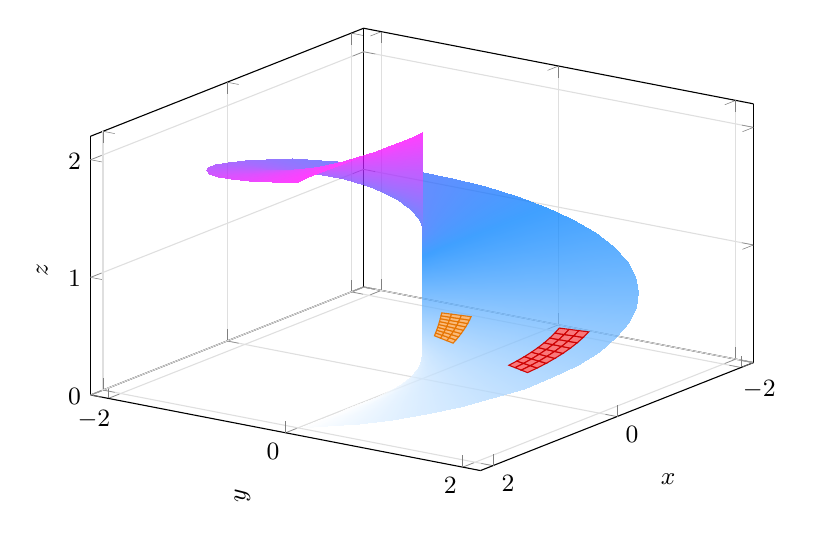
\begin{tikzpicture}
\begin{axis}[width=10cm,height=7.2cm,view={125}{27},axis lines=box,
    xlabel={$x$},ylabel={$y$},zlabel={$z$},
    xmin=-2.2,xmax=2.2,ymin=-2.2,ymax=2.2,zmin=0,zmax=2.2,
    xtick={-2,0,2},ytick={-2,0,2},ztick={0,1,2},
    tick label style={font=\small},label style={font=\small},
    grid=major,grid style={gray!25},domain=0:360,y domain=0:2,
    samples=41,samples y=17,z buffer=sort]
\addplot3[surf,shader=interp,colormap/cool,opacity=.75]
    ({y*cos(x)},{y*sin(x)},{x*pi/540});
\addplot3[surf,shader=flat,draw=orange!90!black,fill=orange!55,
    opacity=.95,domain=70:100,y domain=.2:.5,
    samples=9,samples y=4,z buffer=none]
    ({y*cos(x)},{y*sin(x)},{x*pi/540});
\addplot3[surf,shader=flat,draw=red!80!black,fill=red!55,
    opacity=.95,domain=70:100,y domain=1.4:1.7,
    samples=9,samples y=4,z buffer=none]
    ({y*cos(x)},{y*sin(x)},{x*pi/540});
\end{axis}
\end{tikzpicture}
\end{center}
\endgroup
La figura muestra $a=2$ y $c=1/3$. Los dos parches destacados proceden de rectángulos del mismo tamaño en el dominio $(u,v)$. El parche exterior tiene mayor área porque $\lVert\vec r_u\times\vec r_v\rVert=\sqrt{c^2+u^2}$ aumenta con $u$.

\subsection{Ejercicios}
\begin{enumerate}
    \setlength{\itemsep}{1pt}
    \item Determine cuáles de los siguientes conjuntos pueden describirse globalmente como $z=f(x,y)$. En los demás casos, indique si pueden dividirse en dos gráficas:
\[
z=x^2+y^2,\qquad x^2+y^2+z^2=4,
\qquad x^2+y^2=1,
\qquad z=\sqrt{4-x^2-y^2}.
\]

    \item Para el plano $z=3x-2y+1$, determine el factor que relaciona $dS$ con su proyección $dA$ sobre el plano $xy$. Interprete el valor obtenido en términos de la inclinación del plano.

    \item Calcule el área de la parte del plano $z=x+2y$ situada sobre el triángulo con vértices $(0,0)$, $(2,0)$ y $(0,3)$.

    \item Calcule el área de la parte del paraboloide $z=x^2+y^2$ situada sobre el disco $x^2+y^2\leq4$.

    \item Determine el área lateral del cono $z=2\sqrt{x^2+y^2}$ comprendido entre los planos $z=0$ y $z=6$ mediante su proyección sobre el plano $xy$.

    \item Calcule el área de la parte de la esfera $x^2+y^2+z^2=9$ que se encuentra por encima del plano $z=1$ expresándola como una gráfica sobre el plano $xy$.

    \item La superficie $z=\sqrt{4-x^2}$, $-2\leq x\leq2$, $0\leq y\leq3$, es la mitad superior de un cilindro. Calcule su área mediante la fórmula para gráficas y compruebe el resultado con la fórmula geométrica del área lateral de un cilindro.

    \item Formule, sin evaluar, una integral doble para el área de la superficie $z=xy$ situada sobre el rectángulo $0\leq x\leq2$, $0\leq y\leq1$. Indique por qué el área es mayor que el área de su proyección.

    \item Demuestre que el área de una superficie $z=f(x,y)$ sobre una región $R$ es mayor o igual que $\operatorname{area}(R)$. Determine cuándo ocurre la igualdad.

    \item Considere una región rectangular pequeña de lados $\Delta x$ y $\Delta y$ sobre la que $z=f(x,y)$ se aproxima por su plano tangente. Use dos vectores paralelos a ese plano para justificar la aproximación
\[
\Delta S\approx\sqrt{1+f_x^2+f_y^2}\,\Delta x\,\Delta y.
\]

    \item Para $\vec r(u,v)=\langle u,v,u^2-v^2\rangle$, describa y grafique las curvas coordenadas obtenidas al fijar $u=u_0$ y al fijar $v=v_0$.

    \item Identifique y grafique la superficie $\vec r(u,v)=\langle u\cos v,u\sin v,u\rangle$, $0\leq u\leq2$, $0\leq v\leq2\pi$. Elimine los parámetros para obtener una ecuación cartesiana.

    \item Grafique el helicoide $\vec r(u,v)=\langle u\cos v,u\sin v,v\rangle$, $-1\leq u\leq1$, $0\leq v\leq2\pi$, e identifique la forma de las curvas coordenadas de ambas familias.

    \item Parametrice la parte de la gráfica $z=e^{x+y}$ situada sobre el triángulo $x\geq0$, $y\geq0$, $x+y\leq1$. Especifique el dominio de los parámetros.

    \item Encuentre una parametrización de la parte del cilindro $x^2+z^2=9$ comprendida entre los planos $y=0$ y $y=4$. Elija el orden de los parámetros de modo que el producto $\vec r_u\times\vec r_v$ apunte hacia afuera.

    \item Parametrice la parte de la esfera $x^2+y^2+z^2=a^2$ situada por encima del plano $z=a/2$. Determine los intervalos correctos para los ángulos esféricos.

    \item La curva $y=\sqrt{x}$, $0\leq x\leq4$, gira alrededor del eje $x$. Obtenga una parametrización de la superficie de revolución y calcule su área.

    \item La circunferencia $(\rho-R)^2+z^2=a^2$, donde $R>a>0$, gira alrededor del eje $z$. Construya una parametrización del toro resultante e indique qué representa cada parámetro.

    \item Determine en qué puntos la parametrización $\vec r(u,v)=\langle u^2,v,u^3\rangle$ es regular. Describa qué ocurre con los vectores tangentes cuando $u=0$.

    \item Para la superficie $\vec r(u,v)=\langle u+v,u-v,uv\rangle$, calcule $\vec r_u$, $\vec r_v$ y un vector normal en el punto correspondiente a $(u,v)=(1,0)$.

    \item Encuentre las dos normales unitarias a la superficie $z=xy$ en el punto $(1,2,2)$. Indique cuál tiene componente vertical positiva.

    \item Obtenga el plano tangente a la esfera $x^2+y^2+z^2=14$ en el punto $(1,2,3)$ usando una parametrización local o un vector normal. Compruebe que el vector de posición del punto es perpendicular al plano.

    \item Sea $\vec r(u,v)=\langle u+v,2u-v,3-u+2v\rangle$ sobre $D=\{(u,v):u\geq0, v\geq0, u+v\leq1\}$. Calcule el área de la superficie parametrizada y encuentre su plano tangente.

    \item Use la parametrización $\vec r(u,v)=\langle a\cos u,a\sin u,v\rangle$ para obtener el área lateral de un cilindro de radio $a$ y altura $L$. Explique por qué los extremos $u=0$ y $u=2\pi$ representan la misma curva sobre la superficie.

    \item Para el toro
\[
\vec r(u,v)=\langle(R+a\cos u)\cos v,
(R+a\cos u)\sin v,a\sin u\rangle,
\qquad0\leq u,v\leq2\pi,
\]
donde $R>a>0$, calcule $\lVert\vec r_u\times\vec r_v\rVert$ y demuestre que el área total es $4\pi^2Ra$.

\end{enumerate}
